\chapter{Experimentos Computacionais}

Para a realização do experiemntos computacionais foi necessário, primeiramente, obter os dados para teste e organizá-los para posteriormente submeter ao modelo para geração dos classificadores e aos testes de classificação.

Todo o processo, desde a organização dos dados até a etapa de classificação, foi implementado utilizando a linguagem de programação Java. A implementação foi feita em módulos, organizados da seguinte forma: Módulo organizador dos dados, Módulo de geração de classificadores, Módulo e classificação, Módulo Unificador.

\begin{center}
	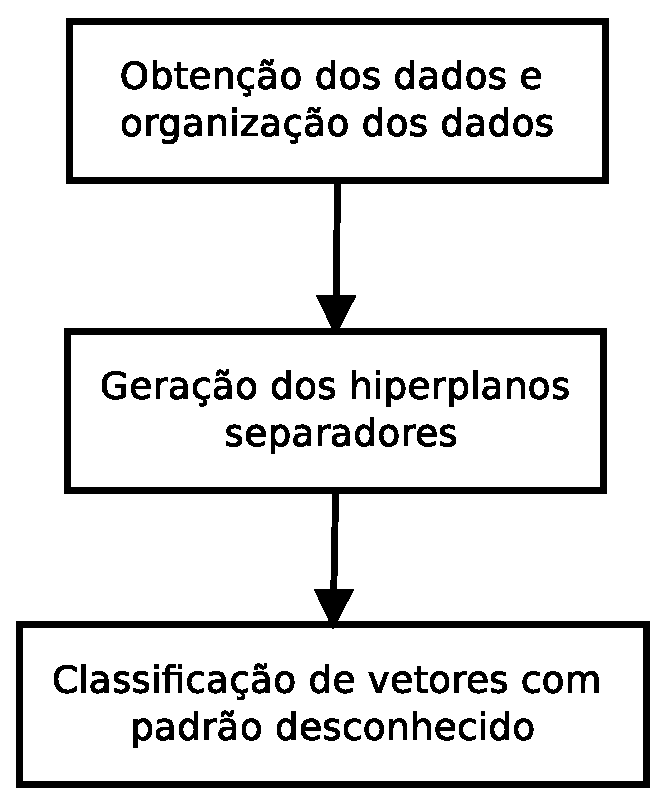
\includegraphics[scale=0.5]{graficos/diagrama_modulos}
	\captionof{figure}{Diagrama simples das etapas reaalizadas nos experimentos}
	\label{img:diagrama_modulos}
\end{center}

Na \ref{img:diagrama_modulos} estão representadas as principais etapas realizadas durante os experimentos computacionais. Primeiramente os dados foram obtidos já no formato de vetores de caracteríticas ou extraídos através de imagens, e depois foram organizados no formato padrão definido para este trabalho. Em seguida foram submetidos ao modelos de Programação Linear, reponsável por gerar os classificadores e por último vetores com padrão desconhecido foram classificados. As duas últimas etapas são repetidas a cada ciclo de teste. Nas seções seguintes essas etapas serão apresentadas de forma mais detalhada.

\section{Conjuntos de Dados}
Foram relaizados testes com quatro conjuntos de dados: dígitos de 0 a 9 escritos manualmente, gestos da Língua Brasileira de Sinais, espécies da planta Iris e expressões facias . Desses conjuntos, os três primeiros foram obtidos do repositório de dados \citeonline{Repositorio2013} e já estavam representados na forma de vetores de características. O último conjunto foi gerado a partir do conjunto de imagens \citeonline{Jaffe}. A seguir são apresentadas as caraterísticas de cada um dos quatro conjuntos de dados:

\begin{itemize}
\item{Dígitos de 0 a 9 escritos manualmente \cite{Digitos}}
Na formação dessa base de dados 250 digítos entre 0 e 9 foram escritos de forma aleatória por 44 pessoas, totalizando 11000 dígitos, porém estão disponíveis 10992 dígitos. Durante a coleta dos dados foram recolhidas, em intervalos fixos de 100 milisegundos, as coordenadas e a pressão da caneta sobre a superfície enquanto o dígito era escrito. Na base de dados utilizada foram considerados apenas os valores das coordenadas. Os dados foram reorganizados utilizando interpolação linear, foram utilizados 8 pontos, e obtidos vetores com 16 características.
Cada vetor é composto por 16 atributos que variam entre 0 e 100 e mais um valor variando entre 0 e 9 que representa o classe representada pelo vetor correspondente.
Os dados estão distribuídos como na tabela a seguir:
\begin{center}
	\begin{tabular}{cc}
        \hline
        Classe & Quantidade de instâncias \\
        \hline
		0 & 1143 \\
		1 & 1143 \\
		2 & 1144 \\
		3 & 1055 \\
		4 & 1144 \\
		5 & 1055 \\
		6 & 1056 \\
		7 & 1142 \\
		8 & 1055 \\
		9 & 1055 \\
        \hline
	\end{tabular}
	\label{tab:tabela_digitos}
        \captionof{table}{Quantidade de instâncias de cada dígito}
\end{center}

\item{Gestos da Língua Brasileira de Sinais (LIBRAS) \cite{Libras}}
Essa base de dados é composta por 15 classes, ou seja, nela estão presentes 15 sinais da LIBRAS, sendo 24 instâncias de cada classe, totalizando 360 vetores de características. Os dados foram extraídos de vídeos com tempo médio de 7 segundos, em cada vídeo um movimento é executado e depois é representado como uma curva bidimensional. No pre processamento foram selecionados 45 frames de cada vídeo, em cada frame a coordenada do ponto central da mão é encontrado, compondo uma curva com 45 pontos. As coordenadas dos 45 pontos formam o vetor de características com 90 valores, os 45 primeiros valores representam o valor de x e o restante o valor de y.
O vetor de características tem no total 91 valores, sendo que 90 deles caracterizam o movimento e o último valor representa o padrão representado pelo vetor.

\item{Espécies da planta Iris \cite{Iris}}
Nessa base dados são representados três tipos da planta Iris, é composta por 50 instâncias de cada tipo, totalizando 150 vetores. Cada vetor é composto por 4 características: comprimento da sépala, largura da sépala, comprimento da pétala, largura da pétala; e mais o nome da classe que o vetor representa.

\item{Expressões facias}
No caso das expressões faciais, as imagens foram obtidas da base de dados \citeonline{Jaffe} e o pre processamento e a extração e caracteríticas foram implementaos na linguagem de programação Python.
Inicialmente ao proposta do presente trabalho era focar apenas na classificação de expressões faciais utilizando a programação linear. Durante a pesquisa não foi encontrada nenhuma base de dados que disponibilizasse os vetores de características da imagens, portanto foi necessária a implementação para a obtenção dos dados. Posteriormente foi verificado que seria necessário um aprofundamento do estudo na área da visão computacional, para que os vetores de caracteríticas não comprometessem o método classificador. Portanto esses dados foram obtidos através de uma implementação superficial de extração de caracteríticas.
Após a obtenção do banco de imagens JAFFE. As imagens foram recortadas a fim de isolar a região da face, utilizando linguagem de programação python, como mostrado na figura

\begin{center}
	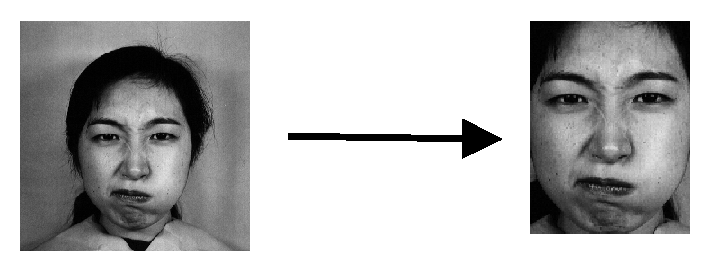
\includegraphics[scale=0.5]{graficos/jaffe}
	\captionof{figure}{Pre processamento das imagens do banco JAFFE}
	\label{img:jaffe}
\end{center}

O banco de imagens JAFFE é composto por 213 imagens, sendo divididas em 7 expressões: tristeza, alegria, desgosto, surpresa, raiva, medo e neutro. Na tebela \ref{tab:tabela_expressoes} é apresentada a quantidade de imagens para cada expressão.

\begin{center}
	\begin{tabular}{cc}
        \hline
        Classe & Quantidade de imagens \\
        \hline
		Tristeza & 31 \\
		Alegria & 31 \\
		Desgosto & 29 \\
		Surpresa & 30 \\
		Raiva & 30 \\
		Medo & 32 \\
		Neutro & 30 \\
        \hline
	\end{tabular}
	\captionof{table}{Quantidade de imagens para cada expressão}
        \label{tab:tabela_expressoes}
\end{center}

Na extração dos vetores de características foi utilizado o método Local Binary Patterns (LBP) que é um classificador de texturas. A cada pixel da imagem é atribuído um código, que é gerado a partir dos pixels ao redor. Tomando como referência o pixel central, a cada pixel vizinho é atribuído o valor 0 ou 1: se o valor do pixel vizinho for menor que o valor do pixel central, o valor 0 é atribuído, se for menor, o valor atribuído é 1. A partir daí, é gerado um código binário que é transformado em um valor decimal, esse valor decimal é o código LBP do pixel central \cite{LBPShan2009}. A figura abaixo demonstra como é calculado o código LBP.

\begin{center}
	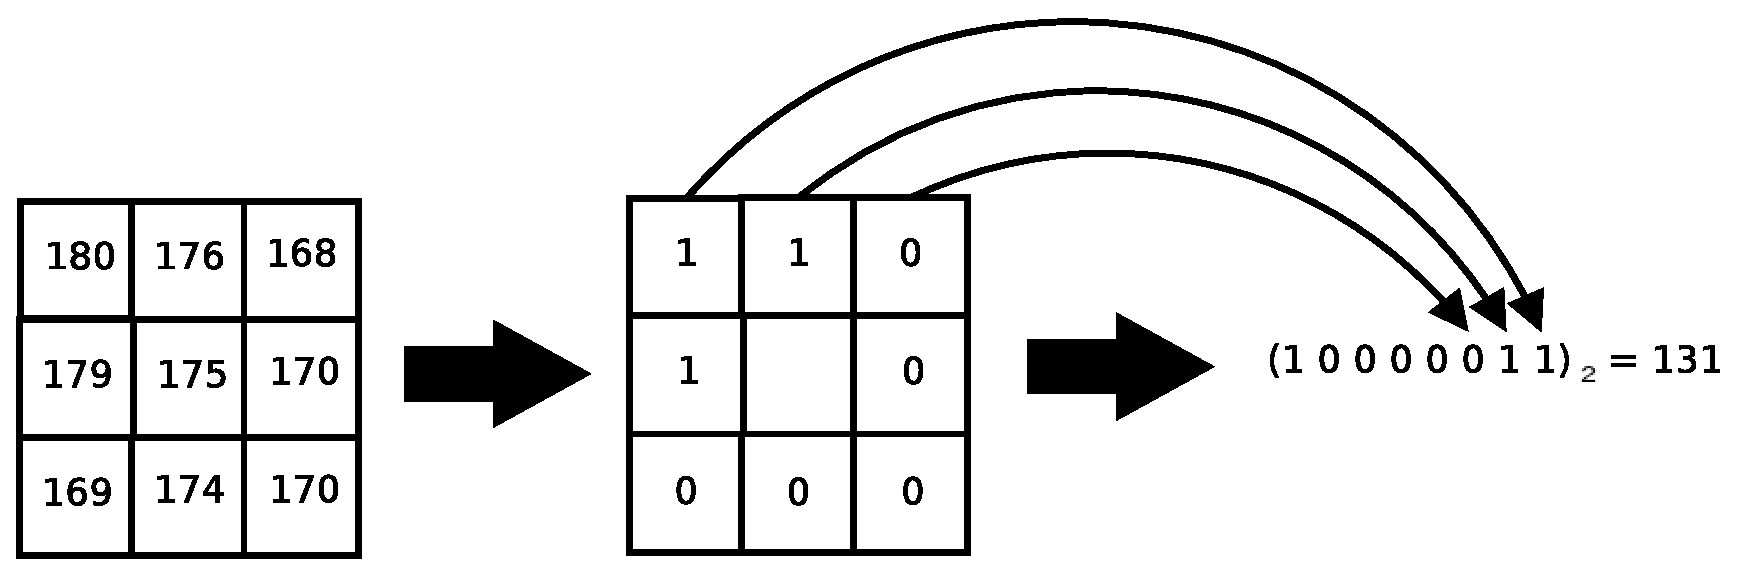
\includegraphics[scale=0.5]{graficos/LBP}
	\captionof{figure}{Cálculo do código LBP}
	\label{img:LBP}
\end{center}

Na implementação, primeiramente, a imagem é dividida em blocos, é gerado o histograma dos códigos LBP de cada bloco, por fim, os histogramas são concatenados. Esse resultado final é o descritor de texturas da imagem. A figura \ref{img:LBPHistograma} representa esse processo.

\begin{center}
	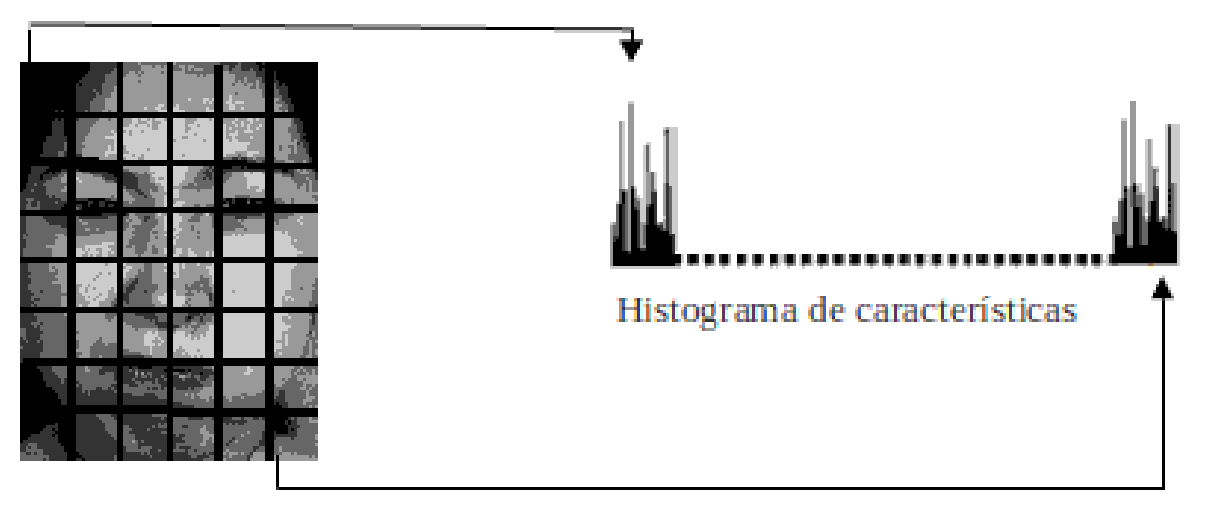
\includegraphics[scale=0.5]{graficos/histograma}
	\captionof{figure}{Representação da imagem dividida em blocos e da concatenação dos histogramas de cada bloco.}
	\label{img:LBPHistograma}
\end{center}

Para reduzir o tamanho do vetor de caracteríticas os códigos LBP de cada pixel são somados e divididos pelo número de imagens, qundo o resultado é menor do que um valor limiar os códigos desse pixel é excluído em todos os vetores \cite{Feng}. O limiar adotado nese caso foi 5 \cite{LBPShan2009}. Resultando em vetores de tamanho 843, sendo composto por 842 caracteríticas mais um dígito identificador do padrão. 
\end{itemize}

Nos vetores de características de todas as bases de dados utlizadas, é acrescido um valor informando a classe representada pelo vetor, para as etapas de treinamento e teste esse valor é omitido, ele só é utlizado na etapa de validação para verificar se o vetor foi corretamente classificado.

\section{Processo de treinamento}
Na etapa de treinamento, os padrões são agrupados em pares e dessa forma são submetidos ao modelo de programação linear, já que o modelo gera um hiperplano que separa dois conjutnos de pontos. Dessa forma para um base de dados com N padrões, a quantidade de pares formados é dada pela fórmula:
$$ \frac{N!}{2\times (N-2)!)} $$

A etapa de treinamento consiste em gerar um hiperplano para cada par formado. No caso da base de dados Iris, por exemplo, que é constituido por 3 classes, são gerados 3 hiperplanos classificadores, da seguinte forma: 
\begin{itemize}
\item{Classificador dos padrões 1 e 2}
\item{Classificador dos padrões 1 e 3}
\item{Classificador dos padrões 2 e 3}
\end{itemize}

Na figura \ref{img:diagrama_modulos} o processo de treinamento corresponde ao módulo de geração de classificadores. Esse módulo foi implementado na linguagem de programação JAVA, utilizada como interface com o software CPLEX da IBM. Os dados necessários para a execução do modelo são lidos de arquivos previamente criados, cada arquivo contêm os dados de uma classe. Os resultados gerados pelo modelo são escritos em um único arquivo, antes dos parâmetros de cada hiperplano, são escritos os padrões dividos pelo hiperplano, como etiquetas identificadoras do hieprplano.
O modelo é resolvido utilizando o método simplex revisado e toda etapa de resolução é feita pelo software CPLEX

\section{Processo de teste}
No processo de teste vetores de caracetrísticas são submetidos a estrtura de áravore de torneio e classificados em um dos N padrões do conjunto de dados.
Na figura \ref{img:diagrama_modulos} corresponde ao módulo de classificação de vetores com padrão desconhecido. E um arquivo contendo vários vetores para teste é utilizado.  A cada teste uma árvore de torneio é construída e um vetor para teste é lido e sua classificação é retornada. Na estrutura de árvore de torneio os padrões são confrotados aos pares, e o hiperplano que separa os dois padrões do par é utlizado para verificar de qual lado do hiperplano o vetor teste se localiza, o padrão que estiver do mesmo lado do vetor teste é elevado ao nível superior da árvore. Para verificar de qual lado o vetor teste de localiza é realizado o seguinte cálculo:

Considerando os padrões A e B, 

Se $ omega \times vetor\_teste < gamma$, o padrão A é elvado ao próximo nível da árvore;

Se $ omega \times vetor\_teste > gamma$, o padrão B é elvado ao próximo nível da árvore; 

\section{Etapa de validação}
Para testar a metodologia utlizada neste trabalho para classificação de padrões, foi utilizado o método cross validation. Através dos resultados desse método é possível analisar a acurácia da metodologia de classificação, ou seja, a capacidade de classificar uma instância com o seu padrão correto.
Entre os três métodos de validação apresentados no referêncial teórico: Handout, Cross Validation e Leave One Out. O método cross validation foi escolhido como melhor opção já que os teste são feitos com várias bases de dados com tamanhos variados. Para bases de dados muito grandes o método Leave One Out de tornaria computacionalmete custoso e o método Handout poderia ter seu resultado comprometido de acordo com os parâmetros escolhidos na separação de dados para teste e de dados para validação. Além disso, o método Cross Validation é de fácil implementação e permite a utlização de todos os dados como teste e validação.
Na figura abaixo o método é ilustrado para o parâmetro 5 fold, apesar desse parâmetro não ter sido utlizado em nenhum teste, foi utlizado para um facilitar a ilustração.
\begin{center}
	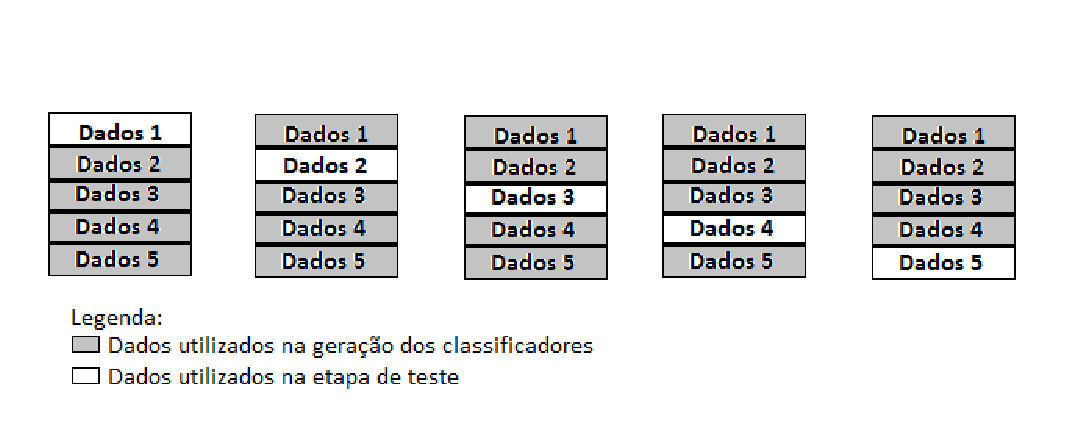
\includegraphics[scale=1.0]{graficos/cross_validation}
	\captionof{figure}{Mecanismo do método de validação 5-fold cross validation}
	\label{img:cross_validation}
\end{center}

Na ilustração o conjunto de dados foi dividido em 5 subconjuntos e consequentemente foram realizados 5 ciclos de treinamento e testes. A cada etapa 4 subconjuntos são utlizados para treinamento e um subconjunto diferente é utilizado para teste. 

A metodologia k-fold cross validation foi implementada na linguagem de programação Java. Os dados são arrumados manualmente em k arquiivos. A implementação seleciona os dados de teste e de validação, e retorna o resultado parcial a cada rodada e o resultado final após os k ciclos de validação e teste. A cada ciclo de treinamento e teste a porcetagem de acerto de classificação é calculada da seguinte forma:

$$A = \frac{acertos}{total}\times 100$$

Onde total é a quantidade de vetores para classificação submetidos a cada ciclo de teste. E acertos é a quantidade de vetores que foram classificados corretamente.

\section{Organização dos dados}
Em todos os testes foi o utilizado o método k -fold cross validation com k = 10, em seus trabalhos \citeonline{Baldisserotto05Validacao}, \citeonline{Kohavi95Cross}, \citeonline{Guo} utlizaram esse mesmo parâmetro. Os dados foram dividos em 10 subgrupos com mesmo tamanho \cite{Guo} e com a mesma quantidade de vetores para cada classe, por isso não foram em utlizados todos os dados de todas as bases de dados.

\begin{center}
	\begin{tabular}{|l|l|l|l|p{3cm}|p{3cm}|p{2cm}|}
        \hline
        Base de dados & Vetores & Vetores utilizados\\ \hline
		Dígitos    &10992  & 10500 \\ \hline
		LIBRAS     & 360   & 300   \\ \hline
		Íris       & 150   & 150   \\ \hline
		Expressões & 213   & 210   \\ \hline
	\end{tabular}
        \captionof{table}{Organização dos dados}
	\label{table:org_dados}
\end{center}

Na tabela \ref{table:org_dados} constam informações das quatro bases de dados utlizadas como teste nomeadas da seguinte forma: Dígitos, LIBRAS, Íris, Expressões. Na segunda coluna são apresentados quantos vetores compõem a base de dados no total sem distinguir o número de vetores por classe. E na última coluna são apresentados o número de vetores utlizados nos testes.

Na base de dados Dígitos, as classes que possuiam menos vetores eram as dos dígitos 3, 5, 8 e 9 com 1055 vetores, e as que possuiam mais vetores eram as dos dígitos 2 e 4 com 1144 vetores como mostrado na tabela \ref{tab:tabela_digitos}. Nessa caso, foram utilizados 1050 vetores de cada classe, totalizando 10500 vetores.

Na base de dados LIBRAS, cada classe possui 24 vetores, para a distribuição dos vetores entre os 10 subgrupos foram utlizados 20 vetores de cada classe, totalizando 300 vetores.

A base de dados Íris possui 50 vetores para cada classe, possibilitando a utlização dos 150 vetores na distribuição entre os 10 subgrupos.

Na quarta base de dados, Expressões, a classe desgosto possui 29 vetores enquanto as classe restantes possuem 30 ou mais, como mostrado na tebela \ref{tab:tabela_expressoes}. Nesse caso, uma imagem da classe desgosoto foi repetida e utilizou-se 30 vetores para cada classe. 

Para essa base de dados Expressões, se vetores fossem excluídos em todas as classes, o número de vetores divisível por 10, que é a quantidade de subgrupos, mais próximo é 20, o que acarretaria a exclusão de 9 ou mais imagens por classe, em contrapartida, na solução utlizada apenas 1 ou 2 imagens foram excluídas de cada classe, com exceção da classe desgosto que teve apenas uma imagem repetida. Já na base de dados Dígitos optou-se pela exclusão, pois seria necessário repetir muitos vetores nas classes com o número mais baixo de vetores, o que poderia comprometer o resultado, o mesmo ocorre com a base de dados LIBRAS.

\section{Resultados}
Nesta seção são apresentados os resultados encontrados nos testes realizados com as quatro bases de dados anteriormento descritas. 

Na tabela a seguir são apresentados os resultados da 4 bases de dados após a validação 10-fold cross validation.

\begin{table}[h!]
	\begin{tabular}{|l|l|l|l|p{2cm}|p{3cm}|p{2cm}|}
        \hline
	Base de dados  & Características & Vetores para treinamento & Vetores para teste & Taxa de acerto (\%)\\ \hline
    	Dígitos    &        16       & 945   & 105 & 0.98\\ \hline
   	LIBRAS     &        90       &  18   &   2 & 0.74\\ \hline
    	Íris       &         4       &  45   &   5 & 0.87\\ \hline
    	Expressões &       842       &  27   &   3 & 0.34\\ \hline
	\end{tabular}
        \captionof{table}{Resultados}
	\label{tab:resultados}
\end{table}

Na tabela \ref{tab:resultados} é aprsentada a quantidade de caracetrísticas presente em cada vetor de cada base da dados, a quantidade de vetores de cada classe utilizados para treinamento e a quantidade de vetores de cada classe utilizados para teste a cada ciclo da validação cruzada. Na última coluna é aprsentada a porcentagem de classificações corretas ao final da validação.

Nessa tabela é possível observar que as classe com menos caracteríticas obtiveram as maiores taxas de acertos. Comparando as duas bases com maioires taxas, observamos que a base Dígitos com um número de vetores muito superior a da base Íris obteve a maior taxa de acerto. A base de dados Expressões, apesar de possuir uma quantidade de vetores superior a da classe LIBRAS, a quantidade de caracteríticas que é um número muito superior e possui a taxa de acerto mais baixa. 

\subsection{Quantidade de vetores X Taxa de acerto}
As bases de dados são compostas por mais de um vetor de características de cada classe, e a quantidade de vetores influência na taxa de acertos final. Para fazer essa análise foi utilizado o banco de dados Dígitos por ser, entre as bases utlizadas, a que contém o maior núemro de vetores por classe.

\begin{table}[h!]
	\begin{tabular}{|l|l|l|l|}
        \hline
	Vetores & Vetores para treinamento & Vetores para teste & Taxa de acerto (\%)\\ \hline
    	   50   & 	45		   &		5	& 	0.898\\ \hline
   	  100   & 	90		   &	       10	&	0.926\\ \hline
	  200   &      180   		   &	       20	&	0.947\\ \hline
    	  300 	&      270		   &	       30	&	0.964\\ \hline
    	  500 	&      450  		   & 	       50	&	0.968\\ \hline
    	  600 	&      540		   &	       60	&	0.972\\ \hline
    	  900 	&      810		   &	       90	&	0.974\\ \hline
    	 1000 	&      900		   &	      100	&	0.975\\ \hline
    	 1050 	&      945		   &	      105	&	0.975\\ \hline
	\end{tabular}
        \captionof{table}{Quantidade de Vetores X Taxa de acerto}
	\label{tab:vetorxtaxa}
\end{table}

Na primeira coluna da tabela \ref{tab:vetorxtaxa} estão específicadas as quantidades de vetores de cada classe e nas duas colunas seguintes as quantidades de vetores de cada classe utilizados na etapa de treinamento e na etapa de testes respectivamente. Na útlima coluna estão específicadas as taxas de acertos em cada teste. 

É possível observar um aumento na taxa de acertos a medida que a quantidade de vetores cresce. Porém esse aumento não é proporcional ao aumento do núemro de vetores. A variação na taxa de acerto diminui a medida que a quantidade de vetores aumenta, do teste com 50 vetores por calsse para o teste com 100, houve um aumento de 2,8\% na taxa de acerto. Já no testes com 200 e 400 a variação na taxa foi de 2\%. E entre o teste com 600 vetores e o teste com quantidade máximamde vetores que é 1050 é observado um aumento bem pequeno de 0,02\% na taxa de acerto.

\subsection{Tempo computacional}
A partir dos testes realizados também foram realizadas análises do ponto de vista computacional.
Todos os experimento foram feitos utilizando um notebbok com configuração core i3 COMPLETAR CONFIGURACAO !!!
Os resultados mostrados na tabela a seguir são as médias dos tempos de 5 execuções.
\begin{table}[h!]
	\begin{tabular}{|l|l|l|l|l|l|l|}
\hline
\multirow{2}{*}{Base de Dados} & \multirow{2}{*}{Classes} & \multirow{2}{*}{Vetores por classe} & \multicolumn{2}{c|}{Tempo de Execução (s)} \\
\cline{4-5}
&&& Gerador de Classificadores & Total\\
        \hline
	%Base de dados  & Classes & Vetores por classe & Gerador de Classificadores & Total\\ \hline
    	Dígitos	       &   10 	 &	1050	      &		  4	           &  37  \\ \hline
   	LIBRAS         &   15 	 &	  20	      &	          1	           &   9,6\\ \hline
    	Íris           &    3	 &        50	      &		 $<1$	           &  $<1$ \\ \hline
    	Expressões     &    7 	 &        30	      &		  1                &  12,4\\ \hline
	\end{tabular}
        \captionof{table}{Tempo Computacional}
	\label{tab:tempocomp}
\end{table}

Na segunda quarta da tabela \ref{tab:tempocomp} estão os temspo de execução apenas do módulo de geração de classificadores, que é o módulo onde o modelo de programação linear é resolvido. É possível constatar um tempo computacional igual ou menor que 1 segundo para três casos, apenas para a base de dados Dígitos esse tempo foi elevado para 4 segundos. Esse aumento pode ser atribuído ao fato de que essa base de dados possui uma quantidae de vetores consideravelmente maior do que as outras bases de dados. Nos experimentos é utlizada a validação 10-fold cross validation, então o módulo gerador de classificadores é executado 10 vezes, porém os tempos expostos na tabela não podem ser multiplicados por 10 para a obtenção do tempo gasto pelo módulo gerador de classificadores em relação ao tempo total da execução porque para a obtenção desses tempos, o módulo foi executado isoladamente e apenas uma vez a cada uma das 5 execuções. \ref{tab:tempocomp}

Na última coluna da tebla \ref{tab:tempocomp} são apresentados os tempos totais de execução de cada experimento. Pode-se constatar que esse tempo é proporcional ao tamanho dos vetores da base de dados e a quantidade de classes. A base de dados Íris obteve um tempo computacional execelente sendo uma base de dados com 3 classe e 50 vetores para cada classe. Enquanto a base de dados Dígitos obteve o maior tempo computacional apesar de possuir vetores com 16 caracteríticas é a base de dados com maior número de vetores por classe. 

Comparando os tempos computacionais das bases Dígitos e Expressões é possível verificar que a quantidade de vetores por classe teve maior influência no tempo de execução, já que a diferença dos tempos de execução das duas classes é bastante alto, proporcional a diferença entre as quantidades de vetores por classe. 

A mesma observação pode ser feita comparando os tempos das base LIBRAS e Expressões, ainda que o núemro de classe da base LIBRAS seja mais que o dobro do número de classes da base Expressões, cada vetor da base Expressões possui 10 características a mais que os vetores da base LIBRAS e o tempo computacional da base Expressões foi superior ao tempo da base LIBRAS.

\section{Análise dos Resultados}

Juntamente com a base de dados Dígitos \cite{Digitos}, estão disponíveis resultados de testes utilizando como metódo de classificação K nearest neighbor, a métrica utlizada para medir as distâncias entro os K vizinhos mais próximos foi a distância Euclidiana. O autor testou variando o parâmetro K de 1 à 11 com a taxa de acerto variando entre 97,34\% e 97,80\%. Em relação ao experimentos realizados neste trabalho é possível verificar que utilizando o método proposto foram obtidas taxas de acertos próximas as encontradas em \citeonline{Digitos}.

Em seu trabalho \citeonline{Swan2012Iris} abordou a classificação de padrões utlizando Redes Neurais e a base de dados Íris. O autor dividiu 75 vetores para treinamento e 75 para teste. Foram realizados 3 testes, variando um parâmetro na configuração da rede neural. As taxas de acertos obtidas variaram entre 83,33\% e 96,66\%. No experiento utilizando o modelo de programação linear a meia de acertos obtida foi de 87\%, um taxa que supera a obtida utilizando redes neurais, dependeno da configuração.

Em \citeonline{Feng} foi utilizada a base de dados JAFFE \cite{Jaffe}. O modelo de programação linear proposto em \citeonline{Bennett92robustlinear} é utlizado para gerar os classificadores e na classificação de imagens com expressão desconhecida foi utilizada uma árvore de torneio, assim como nos experimentos deste trabalho. A taxa de acerto foi de 93.8\%.

No trabalho de \citeonline{Guo} também foi utilizado o banco JAFFE\cite{Jaffe}. Foram feitas comparações entre aluns métodos de classificação, entre eles: Bayes com taxa de acertos 71,0\%, Support Vector Machine linear e não linear, com taxa de acertos 92,4\% e 91,9\%, respectivamente e uma variação do modelo de programação linear utilizado neste trabalho, com taxa 91,0\%. Em todos os casos foram utilizados mecanismos para seleção das características que seriam utlizadas
 
Tanto no trabalho de \citeonline{Feng} quanto no trabalho de \citeonline{Guo} foram obtidas taxas consideravelmente mais altas do que a obtida nos experimentos (34,0\%). Essa diferença pode ser atribuída pela falta de pre processamento das imagens, como já comentado anteriormente.
